%%%%%%%%%%%%%%%%%%%%%%%%%%%%%%%%%%%%%%%%%
% Short Sectioned Assignment
% LaTeX Template
% Version 1.0 (5/5/12)
%
% This template has been downloaded from:
% http://www.LaTeXTemplates.com
%
% Original author:
% Frits Wenneker (http://www.howtotex.com)
%
% License:
% CC BY-NC-SA 3.0 (http://creativecommons.org/licenses/by-nc-sa/3.0/)
%
%%%%%%%%%%%%%%%%%%%%%%%%%%%%%%%%%%%%%%%%%

%----------------------------------------------------------------------------------------
%	PACKAGES AND OTHER DOCUMENT CONFIGURATIONS
%----------------------------------------------------------------------------------------

\documentclass[paper=a4, fontsize=11pt]{scrartcl} % A4 paper and 11pt font size

\usepackage[T1]{fontenc} % Use 8-bit encoding that has 256 glyphs
%\usepackage{fourier} % Use the Adobe Utopia font for the document - comment this line to return to the LaTeX default
\usepackage[english]{babel} % English language/hyphenation
\usepackage{amsmath,amsfonts,amsthm} % Math packages
\usepackage{mathtools} %More math! (For dscases)
\usepackage{hyperref} %HTML package
\usepackage{pgfplots} %Makes plots in LaTeX
\usepackage{tikz} %Also tikz?
\usepackage{bm} %makes vectors bold
\usepackage{bbm} %Blackboard bold 1
\usepgfplotslibrary{fillbetween}%Let's me fill between named plots
\usepackage{graphicx} %import pics
\graphicspath{ {Python_figs/} }
\DeclareGraphicsExtensions{.pdf,.png,.jpg}
\usepackage{sectsty} % Allows customizing section commands
\allsectionsfont{ \normalfont\scshape} % Make all sections the default font and small caps


\renewcommand{\thesubsection}{\alph{subsection}} %Make subsections start with letters
\usepackage{array} % Center in tabular
\usepackage{fancyhdr} % Custom headers and footers
\pagestyle{fancyplain} % Makes all pages in the document conform to the custom headers and footers
\fancyhead{} % No page header - if you want one, create it in the same way as the footers below
\fancyfoot[L]{} % Empty left footer
\fancyfoot[C]{} % Empty center footer
\fancyfoot[R]{\thepage} % Page numbering for right footer
\renewcommand{\headrulewidth}{0pt} % Remove header underlines
\renewcommand{\footrulewidth}{0pt} % Remove footer underlines
\setlength{\headheight}{13.6pt} % Customize the height of the header

\numberwithin{equation}{section} % Number equations within sections (i.e. 1.1, 1.2, 2.1, 2.2 instead of 1, 2, 3, 4)
\numberwithin{figure}{section} % Number figures within sections (i.e. 1.1, 1.2, 2.1, 2.2 instead of 1, 2, 3, 4)
\numberwithin{table}{section} % Number tables within sections (i.e. 1.1, 1.2, 2.1, 2.2 instead of 1, 2, 3, 4)

\setlength\parindent{0pt} % Removes all indentation from paragraphs - comment this line for an assignment with lots of text

\usepackage{listings}
\lstset{language=Python}


%----------------------------------------------------------------------------------------
%	TITLE SECTION
%----------------------------------------------------------------------------------------

\newcommand{\horrule}[1]{\rule{\linewidth}{#1}} % Create horizontal rule command with 1 argument of height

\title{	Assignment 3}

\author{Benjamin Jakubowski} % Your name

\date{\normalsize\today} % Today's date or a custom date

\begin{document}

\maketitle % Print the title

%----------------------------------------------------------------------------------------
%	PROBLEM 2
%----------------------------------------------------------------------------------------

\section*{2. Calculating Subgradients}
\subsection*{2.1 Subgradients for pointwise maximum of functions}

Suppose $f_1, \dots, f_m: \mathbb{R}^d \to \mathbb{R}$ are convex functions. Now let
\[f(x) := \max_{i = 1, \dots, m} f_i(x)\]

Let $k$ be any index for which $f_k(x) = f(x)$ and choose $g \in \partial f_k(x)$. We now show $g \in \partial f(x)$.

Since $g \in \partial f_k(x)$, for all $z$
\[f_k(z) \geq f_k(x) + g^T (z - x)\]
We must show
\[f(z) \geq f(x) + g^T (z - x)\]
Well, since $f_k(x) = f(x)$, we have
\[f_k(x) +g^T (z-x) = f(x) + g^T(z-x) \leq f_k(z)\]
But $f(z) \geq f_k(z)$ (by $f(x) := \max_{i = 1, \dots, m} f_i(x)$), so
\[f(x) + g^T (z - x) \leq f_k(z) \leq f(z)\]
and
\[f(x) + g^T(z - x) \leq f(z)\]
Thus we conclude $g \in \partial f(x)$.

\subsection*{2.2 Subgradients for hinge loss for linear prediction}

First, recall $J(w) = \max\{0, 1- yw^Tx\}$.

We want to find a subgradient of $J$- let's just find the subdifferential. There are three cases:
\begin{itemize}
\item Case 1: If $yw^Tx > 1$, then $J(w) =  \max\{0, 1- yw^Tx\} = 0$. Thus, $J$ is differentiable, and $\nabla J(w) = 0$.
\item Case 2: If $yw^Tx < 1$, then $J(w) =  \max\{0, 1- yw^Tx\} = 1- yw^Tx$. Again, $J$ is differentiable, and $\nabla J(w) = -yx$.
\item Case 3: If $yw^Tx = 1$, then $0 = 1- yw^Tx$. $J$ is not differentiable, so $\partial J(w)$ is the convex hull of $\{0\} \cup \{-yx\}$, which is
\[\{ \alpha_1 \cdot 0 + \alpha_2 (-yx) | \alpha_1, \alpha_2 \geq 0, \alpha_1 + \alpha_2 = 1\} = \{\alpha(-yx) | 0 \leq \alpha \leq 1\}\]
\end{itemize}

%----------------------------------------------------------------------------------------
%	PROBLEM 3
%----------------------------------------------------------------------------------------

\section*{3. Perceptron}
\subsection*{3.1 Perceptron loss on linearly separable $\mathcal{D}$}

Assume $\{x | w^Tx = 0\}$ is a separating hyperplane for a training set $\mathcal{D}$. We show
\[\frac{1}{n} \sum_{i = 1}^n \ell(\hat{y}, y) = 0.\]

First, since we have a separating hyperplane, for all $i, y_i w^T x_i > 0$ (i.e. each training data observation is correctly classified).

Since $\hat{y} = w^T x_i$, for all $i$
\[-\hat{y}_i y_i = -w^T x_i y_i = -y_i w^T x_i < 0\]
So for all $i$, $\max \{0, -\hat{y}_i y_i\} = 0$. Therefore (recalling $\ell(\hat{y}, y) = \max \{0, -\hat{y} y\}$)
\[\frac{1}{n} \sum_{i = 1}^n \ell(\hat{y}, y) = 0\]

\subsection*{3.2 Comparing SGD and the Perceptron algorithm}

If we use SGD to minimize the empirical risk with perceptron loss, with fixed $\alpha = 1$, then our update rule is

\[ w^{(k + 1)} \leftarrow w^{(k)} - \alpha g = w^{(k)} - g \]

where $g$ is a subgradient of our SGD empirical risk function- specifically,

\[
g = 
\begin{cases}
   0 & \textrm{ if } - y_i {w^{(k)}}^T x_i < 0 \\
   -y_i x_i & \textrm{ if not}
\end{cases}
\]

For reference, note that for $- y_i {w^{(k)}}^T x_i > 0, \nabla_w (- y_i {w^{(k)}}^T x_i) =  -y_i x_i$, so (by the same argument as Case 3 in 2.2), $-y_i x_i$ is also a subgradient when $- y_i {w^{(k)}}^T x_i = 0$.

Thus, we can rewrite our update rule as
\[
w^{(k + 1)} \leftarrow 
\begin{cases}
   w^{(k)} - g = w^{(k)} - 0 = w^{(k)} & \textrm{ if }  - y_i {w^{(k)}}^T x_i < 0 \\
   w^{(k)} - g = w^{(k)} - -y_i x_i = w^{(k)} + y_i x_i & \textrm{ if not}
\end{cases}
\]

This is just the Perceptron algorithm given as Algorithm 1 in the assignment (if we cycle through our data points and terminate when training loss is 0, i.e. we've constructed a separating hyperplane).

\subsection*{3.3 Show $w = \sum_{i=1}^n \alpha_i x_i$}

We show this with a simple inductive argument:
At $k = 0$, $w^{(0)} = (0, \dots, 0) \in \mathbb{R}^d$. Then $(y_1x_1^Tw{(k)}) = (y_1x_1^T 0) = 0 \leq 0$,  so 
\[w^{(1)} = w^{(0)} + y_i x_i = 0 + y_i x_i = y_i x_i\]

Now consider the $(k + 1)^{st}$ step (made on the $j^{th}$ data point). Assume $w^{(k)} =  \sum_{i=1}^n \beta_i x_i$. Consider our update:
\[
w^{(k + 1)} \leftarrow 
\begin{cases}
   w^{(k)} & \textrm{ if }  - y_j {w^{(k)}}^T x_j < 0 \\
   w^{(k)} + y_j x_j & \textrm{ if not}
\end{cases}
\]

Since $w^{(k)}$ is a linear combination of the $x_i$'s, it's obvious $w^{(k+1)}$ is as well.

Next, assume the algorithm terminates and returns $w = \sum_{i=1}^n \alpha_i x_i$.

By construction, it is apparent
\[
\alpha_i 
\begin{cases}
   = 0 & \textrm{ if } x_i \textrm{ was correctly classified by every } w^{k} \textrm{ such that } k \bmod n = i - 1 \\
   \neq 0 & \textrm{ if } x_i \textrm{ was incorrectly classified by some } w^{k} \textrm{ such that } k \bmod n = i - 1
\end{cases}
\]

%----------------------------------------------------------------------------------------
%	PROBLEM 4
%----------------------------------------------------------------------------------------

\section*{4. The Data}
\subsection*{4.1 Load and randomly split the data (75-25 training-test)}

See attached iPython notebook.

%----------------------------------------------------------------------------------------
%	PROBLEM 5
%----------------------------------------------------------------------------------------

\section*{5. Sparse Representations}
\subsection*{5.1 Write a function that sparsifies an input list of words}

See attached iPython notebook.


%----------------------------------------------------------------------------------------
%	PROBLEM 6
%----------------------------------------------------------------------------------------

\section*{6. Support Vector Machine via Pegasos}
\subsection*{6.1 Compute a subgradient for the "stochastic" SVM objective}

The "stochastic" SVM objective is
\[h_i(w) = \frac{\lambda}{2} ||w||^2 + (1 - y_i w^T x_i)_+\]

Now, note we have three cases (either side or at the non-differentiable point):

\begin{itemize}
\item For $y_i w^T x_i < 1, h_i(w) = \frac{\lambda}{2} ||w||^2 + (1 - y_i w^T x_i)$. This is differentiable with respect to $w$, so $\partial h_i(w) = \{ \nabla_w h_i\} = \{\lambda w - y_i x_i \}$. Thus, the update rule (with $\eta_t = 1 / (\lambda t)$) is
\begin{align*}
w_{t+1} &\leftarrow w_t - \eta_t g \\
	&\leftarrow w_t - \eta_t (\lambda w - y_i x_i) \\
	&\leftarrow (1 - \eta_t \lambda) w_t + \eta_t  y_i x_i
\end{align*}
\item For $y_i w^T x_i > 1, h_i(w) = \frac{\lambda}{2} ||w||^2$, so $\partial h_i(w) = \{ \nabla_w h_i\} = \{\lambda w\}$. Thus, the update rule is
\begin{align*}
w_{t+1} &\leftarrow w_t - \eta_t g \\
	&\leftarrow w_t - \eta_t \lambda w \\
	&\leftarrow (1 - \eta_t \lambda) w_t
\end{align*}
\item For $y_i w^T x_i = 1$, we have $\partial h_i(w) = \textbf{Conv} \{\lambda w\} \cup \{\lambda w - y_i x_i \}$. Thus, $\lambda w$ is itself a subgradient, and 
\begin{align*}
w_{t+1} &\leftarrow w_t - \eta_t g \\
	&\leftarrow (1 - \eta_t \lambda) w_t
\end{align*}
\end{itemize}

\subsection*{6.2 Implement the Pegasos algorithm}

See attached iPython notebook.

\subsection*{6.3 Implement the improved Pegasos algorithm}

The initial implementation of the Pegasos algorithm is very slow, since at each stochastic step we must update every entry in the weight vector (which is a large dictionary).

Thus, to decrease runtime, we can represent $w$ as $w = sW$, where $s \in \mathbb{R}$ and $w \in \mathbb{R} ^d$.

First, we verify this- note it is obvious that the update $w_{t+1} = (1 -  \eta_t \lambda) w_t$ is equivalent to
\begin{align*}
W_{t+1} &= W_{t} \\
s_{t+1} & =  (1 -  \eta_t \lambda) s_t
\end{align*}
Thus, we show the update $w_{t+1} = (1 -  \eta_t \lambda) w_t + \eta_t y_j x_j$ is equivalent to
\begin{align*}
s_{t+1} &= (1 - \eta_t \lambda) s_t \\
W_{t+1} & = W_t + \frac{1}{s_t + 1} \eta_t y_j x_j
\end{align*}

First, note
\begin{align*}
w_{t+1} &= s_{t+1}W_{t+1} \\
\frac{w_{t+1}}{s_{t+1}} & = W_{t+1} \\
\frac{(1 - \eta_t \lambda) w_{t} + \eta_t y_i  x_i}{s_{t+1}} & = W_{t+1}
\end{align*}
Now, letting $s_{t+1} = (1- \eta_t \lambda) s_t$ yields

\begin{align*}
\frac{(1 - \eta_t \lambda) w_{t} + \eta_t y_i  x_i}{(1- \eta_t \lambda) s_t} &= W_{t+1} \\
\frac{(1 - \eta_t \lambda) w_{t}}{(1- \eta_t \lambda) s_t} +  \frac{\eta_t y_i  x_i}{(1- \eta_t \lambda) s_t} &= W_{t+1} \\
W_t + \frac{1}{s_{t+1}} \eta_t y_j x_j &= W_{t+1}
\end{align*}

Thus, representing $w = sW$ allows us to update much more quickly (on the order of the number of non-zero entries of $x_j$).

\subsection*{6.4 Running and comparing both versions of the Pegasos algorithm}

Both versions of the Pegasos algorithm were run for 10 iterations (with $\lambda$ set to 0.1), and the final weight vectors $w$ and runtimes were compared. First, the runtimes are given below:

\begin{center}
\begin{tabular}{| p{6.6cm} | c |}
\hline
\textbf{Version of Pegasos} & \textbf{Runtime} \\
\hline
First version (naive representation of $w$)\newline including check for convergence & \texttt{1 loops, best of 3: 9min 4s per loop} \\
\hline
Second version (representing $w = sW$)\newline not including check for convergence & \texttt{1 loops, best of 3: 4.12 s per loop} \\
\hline\hline
Second version (representing $w = sW$)\newline including check for convergence & \texttt{1 loops, best of 3: 7.18 s per loop} \\
\hline
\end{tabular} \\
\end{center}

Obviously the second version of the algorithm is a dramatic improvement over on the first. Next, to confirm the two results return essentially the same weight vector, the relative differences in weights are reported.

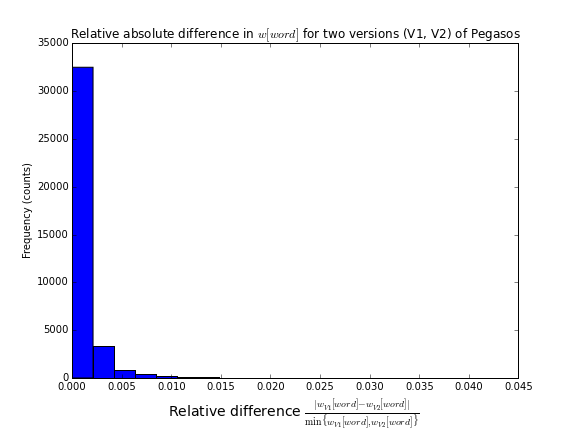
\includegraphics[scale = 0.65]{./../figures/6_4.png}

It is apparent from the small relative differences that these two implementations are returning essentially the same weight vector (up to differences errors attributable to floating point precision on $1500 \times 10 = 15000$ updates to the weight vector $w$).

\subsection*{6.5 0-1 loss of linear predictor $x \mapsto w^Tx$}

See attached iPython notebook

\subsection*{6.6 Optimizing $\lambda$}

To find the optimal $\lambda$, the average validation set 0-1 loss was calculate for the SVM model fit with $\lambda$ in $\{10^{-7}, 10^{-6}, \dots, 10^3\}$.

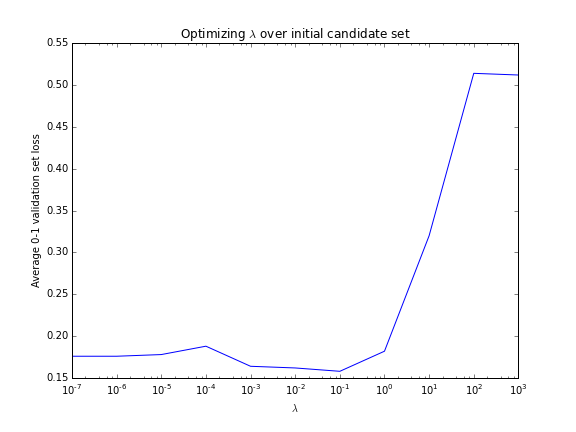
\includegraphics[scale = 0.65] {./../figures/6_6_a.png}

Based on model performance across this range, further exploration was conducted over the subsets of this range. Ultimately, the optimal $\lambda$ value was found to be 0.14.

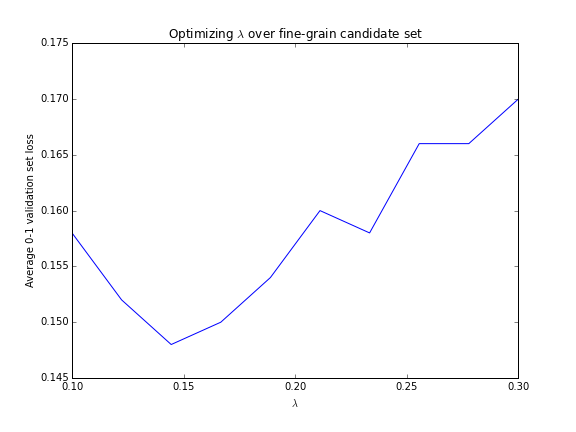
\includegraphics[scale = 0.65] {./../figures/6_6_b.png}

\subsection*{6.7 Comparing scores (i.e. $f(x) = w^T x$)}

In SVM, we assume the score corresponds to the confidence of our prediction. To test this assumption, we compare the scores of true positive and negative instances from our validation set. First, histograms showing the scores for these subsets are shown below:

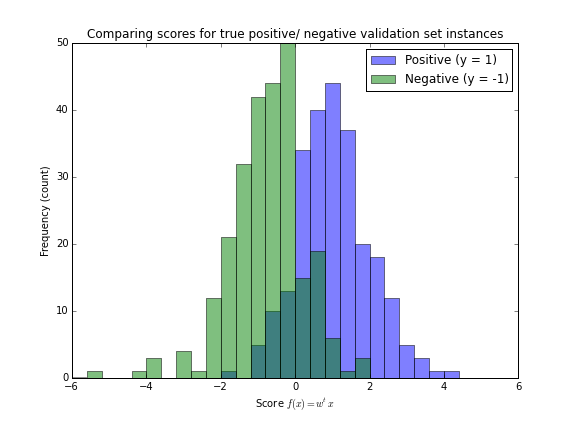
\includegraphics[scale = 0.65] {./../figures/6_7_a.png} 

Next, the estimated probability of error was determined for each bin (using the relative frequency of misclassified instances). These  probability estimates are shown in the plot below- note the size of the point corresponds to the number of instances in the bin. \\

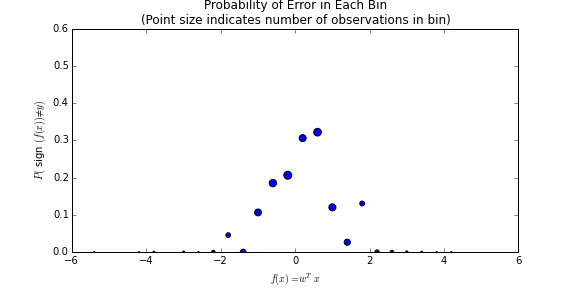
\includegraphics[scale = 0.65] {./../figures/6_7_b.png}

From this plots, it's apparent that the score does in fact correspond to the confidence of our prediction (since the conditional probability of error given a large absolute scores is low).

\subsection*{6.8 Investigating the case $y_iw^T x_i = 1$}

Our hinge loss function is not differentiable when $y_iw^T x_i = 1$. However, it is worth asking how often and when we hit this point. In our training data, we find 0 training set points with $y_iw^T x_i = 1$ This makes sense- $w$ is a vector in $\mathbb{R}^{38793}$, with floating point entries. Thus, the probability of constructing a text string such that $y_iw^T x_i = 1$ is extremely low.


%----------------------------------------------------------------------------------------
%	PROBLEM 7
%----------------------------------------------------------------------------------------

\section*{7. Error Analysis}

The follow approach was taken to analyze errors made by our model:
\begin{enumerate}
\item First, incorrectly classified instances were ranked by the absolute score to identify the 10 "biggest" mistakes.
\item Then, for each of these 10 mistakes, the 10 features that contributed most heavily (i.e. largest $|w_i x_i|$) to the decision were identified and listed.
\end{enumerate}

These mistakes are listed below:
\begin{center}
\lstinputlisting[language={}, basicstyle=\ttfamily\small]{./../error_examples.txt}
\end{center}

There are two observations we can make from these errors.
\begin{enumerate}
\item First, it's apparent frequent words are decreasing the performance of the model. Specifically, a number of high-frequency words are assigned small weights (example: \texttt{the} is assigned the weight 0.0031). While the weights are small, the frequency of these words is high in many documents, and as a result they can produce errors.
\item In addition, the model is unable to account for context-dependent differences in the meaning of words like \texttt{bad} and \texttt{good}. These words can be negated (or otherwised used in contexts that change meaning), and (given these words are assigned large negative weights, i.e. $w\texttt{[bad]} = -0.1391$) this can lead to errors.
\end{enumerate}

To try to address these errors, two feature engineering approaches will be tested. First, we will test model performance after introducing bigrams. This is hypothesized to reduce error due to negation of heavily weighted terms (i.e. account for \texttt{not good}). Second, we will test model performance using a TF-IDF feature set (for the bag-of-words and bigram representation). This is hypothesized to reduce the impact (via IDF weighting) of high frequency terms (like \texttt{the}).



%----------------------------------------------------------------------------------------
%	PROBLEM 8
%----------------------------------------------------------------------------------------

\section*{8. Features}

\subsection*{8.1 and 8.2 New features}

As described above, we will attempted to improve performance using the following feature:
\begin{enumerate}
\item 1-grams (previously conducted)
\item 1-grams and bigrams.
\item TF-IDF for 1-grams
\item TF-IDF for 1-grams and bigrams
\end{enumerate}
We present histograms showing the distribution of scores for the true positive and true negative ratings, as well as the estimated probabilities of errors (including 95\% confidence intervals on this probability).

\begin{center}
\begin{tabular}{| m{3cm} | m{8cm} | m{3cm} |}
\hline
	\textbf{Feature set} & \textbf{Distribution} & \textbf{Average 0-1 loss}\newline($\hat{p}, \hat{p} \pm 1.96 \cdot SE$) \\
\hline
	1- and 2-grams\newline(counts) & 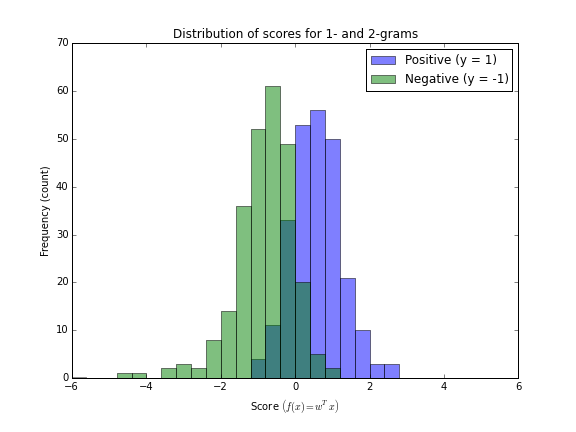
\includegraphics[scale=0.4]{./../figures/8_2_a.png} & 0.15 \newline (0.1187, 0.1813) \\
\hline
	1-grams\newline(TF-IDF) & 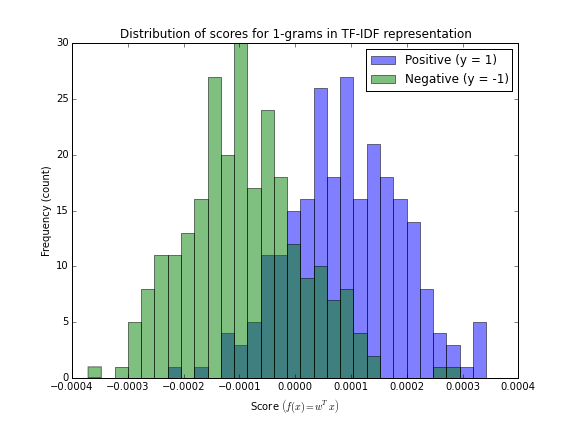
\includegraphics[scale=0.4]{./../figures/8_2_b.png} & 0.188 \newline (0.1538, 0.2222) \\
\hline
	1- and 2-grams\newline(TF-IDF) & 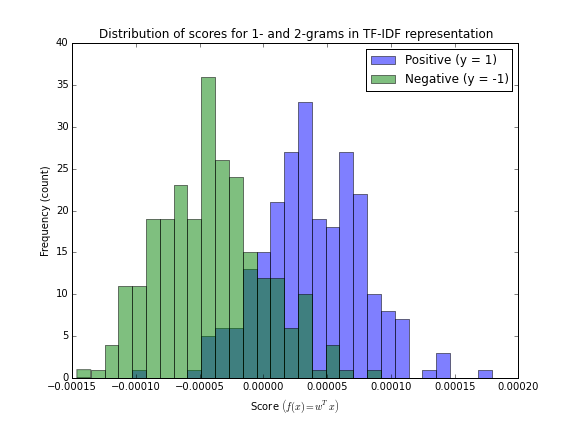
\includegraphics[scale=0.4]{./../figures/8_2_c.png} & 0.166 \newline (0.1334, 0.1986) \\
\hline
\end{tabular}
\end{center}

Unfortunately, it does not seem that any of these alternate feature sets or representations produced an improved model (i.e. model with lower out-of-sample average 0-1 loss). Note, however, $\lambda$ was not optimized for these alternate models. If additional time was available, I would have first searched for an optimal lambda value for each of these feature spaces, then determined the validation set 0-1 loss for this optimized model.

Still, given the results available, it appears the best model is the original 1-gram model (both in terms of runtime and average 0-1 loss).
%----------------------------------------------------------------------------------------


\end{document}